\title{2023 Research Status Report: Infrared Stellar Occultation Studies of Saturn's Atmosphere from Cassini VIMS}
\author{An}
\date{\today}

\documentclass[12pt]{article}
\usepackage[margin=1in]{geometry}
\usepackage{graphicx}
\usepackage{natbib}
\graphicspath{{.}}


\begin{document}
\maketitle

\begin{abstract}

I started grad school in Fall 2016.  I settled on an advisor and began scoping
out and understanding this project in the Fall of 2018.  In the Spring of 2019,
I applied for and was awarded this grant over the Summer. I began work in the
Fall of 2019.  During that time, I created a preliminary analysis of the
imaging-mode occultations as a launchpad for the rest of the analysis.  In
January of 2020, I put the grant on hiatus to help an emergency management
start up.  The grant resumed in 20 August 2022. I have been reacquainting myself
with the field of astronomy, my skills in physics, and my previous work.  This
progress report represents my analysis of the work that I did during this
grant's previous active period, my plans to complete the promised analysis of
the Cassini VIMS occultation data per my proposal, a discussion of planned
publications using these data to constrain models of Saturn's atmospheric
chemistry, applications to understanding photochemistry in exoplanet
atmospheres, applications to brown dwarf atmospheres, applications to
astrobiology, applications to Uranus, and applications to Titan research.

\end{abstract}

\section{Administrative}

Title of Grant: Stellar Occultation Studies of Saturn’s Atmosphere\\
Type of Report: Progress Report\\
Name of the principal investigator: Philip Nicholson\\
Period Covered by the report: 2022-08-20 to 2023-03-15 \\
Cornell University, 418 Space Sciences Building, Ithaca, NY 14853\\
Grant Number: 80NSSC19K1528\\

\section{Data Analysis: Objectives and Accomplishments}

Cassini VIMS observed over 100 occultations by Saturn of background stars, a
handful of which were observed through a series of small-frame images instead
of a single spatial pixel pointed at the star's initial location on the sky.
These imaging-mode occultations provide a chance to directly observe the stars'
refraction through the outer layers of Saturn's atmosphere and constrain the
relative importance of differential refraction to other sources of attenuation
in the photometry of an occultation. This is an important calibration for the
higher-radial-resolution occultation-mode data, for which the image of the star
much more quickly gets refracted out of the field of view.

\begin{figure}[h!]
  \centering
  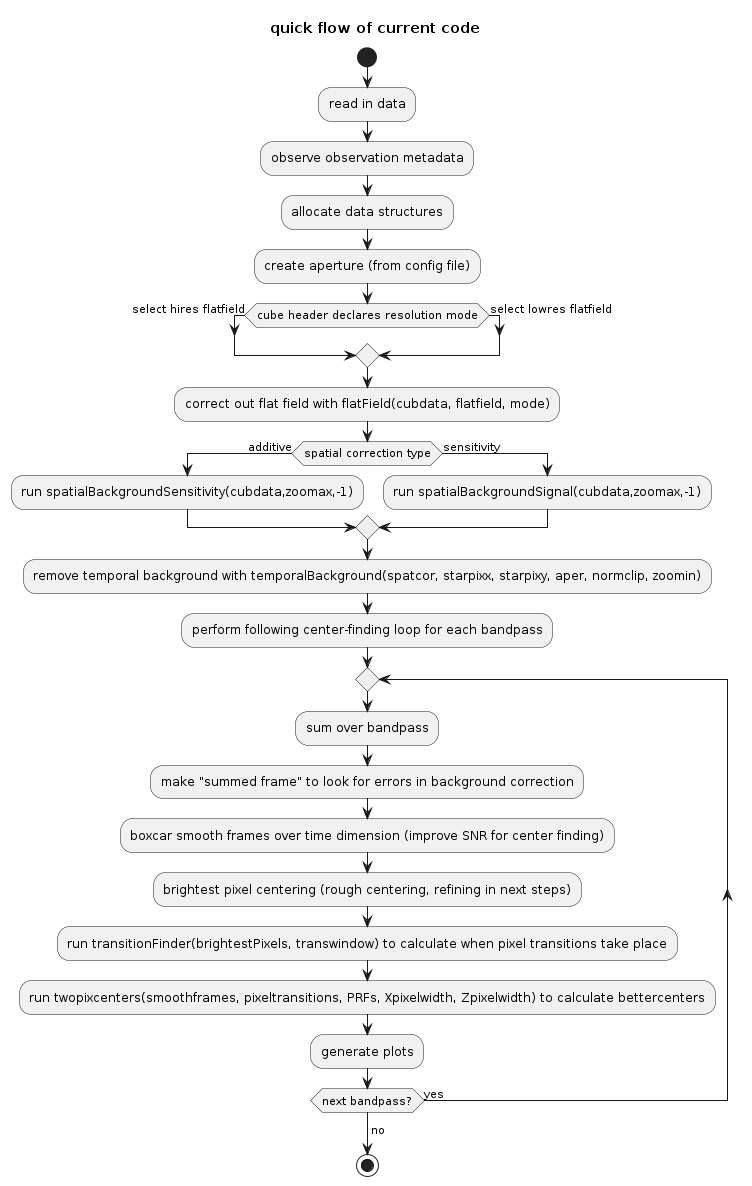
\includegraphics[width=0.7\linewidth]{codeflow.png}
  \caption{code flowchart for current version}
  \label{fig:codeoverview}
\end{figure}

As such, my initial analysis targeted these imaging-mode occultations.  I wrote
a code that looks like Figure \ref{fig:codeoverview}. It corrects out known
sources of noise and performs standard aperture photometery. It produces
lightcurves, X and Z centering results to track the star getting refracted out
of frame, differences in the star's center by wavelength, spectra, and movies
of these properties during the event, an example can be seen in Figure \ref{fig:codeplots}

\begin{figure}[h!]
  \centering
  \includegraphics[width=0.95\textwidth]{codeplot.png}
  \caption{Lightcurve and centering results for an occultation of AlpOri
(Betelgeuse) on orbit 271, observed in the 2.7~$\mu$m continuum band. The top
plot displays the flux dropping and twinkling through the atmosphere. The
bottom plot displays the centroid location calculated for the star, plotted
over a line with a slope matching the spacecraft's velocity. This is one of
four types of plots produced by the code. See the code outline document for
more details.}
  \label{fig:codeplots}
\end{figure}

There are four major tasks of the code. Two of them have been implemented in
some form, and are iterating towards completion. These two act on only the
imaging-mode data. The two tasks remaining to write act on all data.

\subsection{Background Subtraction}

The standard aperture photometry methods employed are insufficient for these
data. There isn't always a "sky", and the background level changes as the limb
of the planet enters and then engulfs the field of view.  A more honest
background correction needs to model this moving limb of the planet as having a
different background flux for each frame's background correction. Discussions
on implementing this have begun. Detail on the current implementation can be
found in the code outline document. For now, we are not yet ready to describe
the new background correction in detail.

\subsection{Centering Algorithm}

See the Centering document for a full discussion.

Tracking the center of a star in a VIMS image is a difficult task because the
PSF of the star is less than one pixel. Still, the star is rarely centered in a
pixel, and so centering can be achieved by looking at how much light spills
into the neighbors of the brightest pixel. Fortunately, the Pixel Response
Function (PRF) is well-defined for the single VIMS spatial pixel as a function
of the angle between the center of the pixel and the star. This has been done
by slewing the spacecraft so that the star AlpOri (Betelgeuse) raster-scans
across the pixel. From these, we can calculate the theoretical relative
brightnesses of the pixels on either side of the brightest pixel relative to
the brightest pixel, and compare this to the measured value in the VIMS frame.


First, we must determine which two pixels share the most starlight. To do so,
we:
\begin{enumerate}
  \item integrate over a continuum bandpass to improve signal to noise (e.g. 2.53-2.85 microns)
  \item perform a boxcar smoothing in time (usually 10 frames)
  \item record the brightest pixel for each resulting timestep
  \item locate "transition times" when the brightest pixel changes from one timestep to the next
  \item at each timestep select the brightest pixel and the brightest pixel on the other side of the nearest "transition"
\end{enumerate}

We measure the direction to the star by taking the ratio ($R_{data}$) of the
de-noised signal in these two selected pixels.  We compare this ratio to the
same ratio calculated from the PRF scans $R_{scans}(t)$ at each time step $t$.
We calculate the value of $t=t_0$ for which $\chi^2 =
(R_{data}-R_{scans}(t_0))^2$ is minimized, and then calculate $\theta(t_0)$
which is the offset of the star from the center of the pixel at $t_0$. 

\begin{equation}
R_{data}^x = \frac{P^{x\pm1}}{P^{x}}
\end{equation}

And in the $z$ direction this ratio is defined as:

\begin{equation}
R_{data}^z = \frac{P^{z\pm1}}{P^{z}}
\end{equation}

Where $P^x = P^z$ is the brightness of the brightest pixel (integrated over
some wavelength range), and $P^{x\pm1}$ and $P^{z\pm1}$ are those of the
adjacent pixels in each direction.

This metric has many properties which make it useful. Theoretically, it should
be monotonically increasing or decreasing as the star position increases
steadily in pixel position.  For PSFs smaller than a pixel, there will be a
plateau at zero where there is no light observed in the neighboring pixel. Away
from this plateau (near the pixel boundaries) we have the best sensitivity to
the position of the star. At metric values $R = 1$ the center of the star's PSF
straddles the boundary with the neighboring pixel and we have the most
sensitivity.

{\bf The current version of the code performs fits in each direction independently,
and using manually-selected PRF scan track numbers. A planned improvement is to
fit both simultaneously, which will allow the algorithm to self-select the best
track for each direction.} 

After this step, we have occultation profiles in the same form as the
occultation-mode data. This ends the imaging-mode specific portion of the code.
The following two subsections describe code that will be run on all occultation
data.

\subsection{Calculating Temperature and Pressure from Refraction in the Continuum Bands}

The current version of the code does not yet perform this calculation.

Consider a light ray from the occulted star incident on a spherical planet of
radius $R$, at an impact parameter $\rho$. As it penetrates more deeply into
the atmosphere, where the refractive index of the gas is larger, the ray
gradually refracts towards the planet's center until it reaches a minimum
radius, after which it traces a mirror-image path back out of the atmosphere.

The formal expression for the overall angular deflection of the ray once it
emerges from the atmosphere is:

\begin{equation}
 \theta(\rho) = -2\rho \int_{r_0}^\infty \frac{dn/dr}{n\sqrt{n^2r^2 - \rho^2}}\, dr,
\end{equation}

\noindent where $n(r)$  is the refractive index profile of the atmosphere,
and the ray's minimum radius $r_0$ is specified by the condition $n(r_0)r_0 = \rho$.

Adjacent light rays are deflected by progressively larger amounts as $\rho$
decreases and the rays penetrate more deeply into the atmosphere. As a result
of this {\it differential refraction}, the flux of light from the source is
reduced by a factor of $\Phi$:

\begin{equation}
 \Phi(\rho) = \left( 1 - D\frac{d\theta}{d\rho} \right)^{-1}\left( 1 - \frac{D\theta}{\rho} \right)^{-1},
\label{eq:iso_flux}
\end{equation}

\noindent where $D$ is the distance from the planet to the observer. The second
factor represents the focusing effect that occurs near the center of the
geometric shadow and can be neglected for our data where $D\theta\ll\rho$.

As described in \cite{Elliot77} and \cite{French78}, we can use these two
expressions to perform an inverse Abel transform and invert our occultation
lightcurves in regions of the spectra dominated by differential refraction to
acquire multiple {\bf radial profiles of the temperature and pressure in the
planet's stratosphere.}

This technique is standard for inversions of differential-refraction dominated
stellar occultations.  Due to Saturn's highly oblate shape, the above
expressions are adjusted in practice to use a local spherical fit to the
atmosphere.

We are confident that the attenuation of the starlight at wavelengths where
hydrocarbon molecular absorption is negligible is dominated by the
above-described impact of differential refraction and not aerosol-driven
scattering extinction. Although aerosols are an important chemical component of
Saturn's atmosphere, these particles are likely sub-micron in size and their
scattering efficiency should decrease rapidly with decreasing wavelength,
perhaps scaling as $\lambda^{-q}$ where $q$ is between 1 and 4. The aerosols on
Titan follow such a power law with $q\simeq1.8\pm0.5$ \citep{Bellucci09}. The
extinction in the VIMS Saturn occultations at wavelengths outside of the strong
hydrocarbon bands is observed to be essentially {\sl independent} of
wavelength, strongly suggesting that aerosol extinction is negligible at the
few mbar level and above and therefore we may neglect them in our models. {\bf
One goal of the imaging-mode occultations is to test this assumption by
following the star much deeper into the occultation than is available in
occultation-mode, and directly measuring the bending angle (distance the image
has moved across the detector) and the flux to compare to values predicted by
the above equations.}

\subsection{Calculating Molecular Abundances from Spectra}

The current version of the code does not yet perform this calculation.

Let's consider an "onion-skin" model of an atmosphere for which each thin
radial layer is of uniform composition and density. As a ray of star light
passes through each of these layers, it is attenuated according to the
equation:

\begin{equation}
\Phi(\lambda) = \Phi_0\ e^{-\delta\tau(\lambda)},
\label{eq:abs_flux}
\end{equation}

\noindent where $\Phi_0$ is the attenuation experienced before entering that layer
and $\delta\tau(\lambda)$ is the optical depth of the layer as a function of
wavelength, described by the equation:

\begin{equation}
\delta\tau(\lambda) = \kappa(\lambda) L d
\label{eq:optical_depth}
\end{equation}

\noindent Here, $\kappa$ is the absorption coefficient, $L$ is the slant
pathlength, and $d$ is the density of the layer which is known from the
inversion of the lightcurve at the refraction-dominated continuum wavelengths.

The data for a given occultation can be thought of as a time-series of spectra,
each of which cuts a deeper path through the atmosphere than its predecessor.
Each time-step can be used to constrain the opacity of an additional deeper
layer, and then be used as an input to the next timestep since that layer will
also be probed during the subsequent observations. Datapoints can be binned in
time to increase signal to noise at the expense of the radial resolution of the
resulting abundance profile. We call this technique "onion-peeling" and a
preliminary proof-of-concept using a single wavelength bin was presented by
\cite{Banfield11}.

We will fit a model to a full-spectrum $\kappa(\lambda)$ calculated in each
layer from our data. A model spectrum will be calculated with a line-by-line
approach using Voigt profiles calculated using the pressures and temperatures
from our refraction inversions described above.  We will use line list
databases such as the HITEMP database from HITRAN
\footnote{https://hitran.org/hitemp} \citep{Gordon17b} for each gas relevant to
Saturn's atmosphere. The contributions of each gas (chiefly CH$_4$ and
C$_2$H$_6$, but possibly also C$_2$H$_2$) to the final opacity are independent
and proportional to their mixing ratios, which will be fit to the data.

In practice, hydrogen and helium are essentially transparent in the
near-infrared for any reasonable path length through the stratosphere
\footnote{H$_2$ does have a fundamental vibrational transition at 2.1~$\mu$m,
which is detectable in the spectra of the Jovian planets, but this is a
collision-induced absorption that scales as  $p^2$, and so is very weak in the
stratosphere, even for very long path lengths.}  so the opacity is dominated by
trace gases, methane, ethane, and acetylene \citep{Moses05}.

\section{Status Changes and Budget}

Should I request travel funding to DPS or the Uranus workshop?

\section{Results to Eventually Disseminate}

I need help to flesh these out. I will use these bullets as a starting point to
help me find committee members.

\begin{itemize}
  \item Overview of Cassini occultation data analysis
  \item Seasonal variations of photochemistry. This effect is visible by eye, and should be quantifiable with our data.
  \begin{itemize}
     \item Comparison to \citep{Fletcher10} CIRS observations where CH4 distribution could not be uniquely determined from CIRS alone. See if we can help break that degeneracy?
     \item Comparison to \citep{Moses05} and \citep{Fouchet09} 1-D chemistry models
     \item Tying these models to the canonical D.F. Strobel 1969 paper on the
      "methane cycle", and updating that framing
     \item Comparison to predictions from various exoplanet atmospheric models that
      are currently "in vogue"? How well do these models fit the atmosphere of
      an endoplanet? Should we test them directly while peeling the onion?
     \item Comparison to what we know about / expect to find in Uranus???
  \end{itemize}
  \item Paper on the chemistry of aerosols produced at the end-stage of photochemistry
  \begin{itemize}
     \item sedimentation, nucleation, cloud-seeding \citep{Fletcher18}
     \item astrobiological implications?
     \item What can we say about complex organics sedimenting down into a region of
      convective ammonia cloud condensation? What kinds of amino-organic
      compounds might they form?
     \item compare to titan chemistry?
  \end{itemize}
\end{itemize}

What originally got me interested in this project was the relationship to
photochemistry models in exoplanet atmospheres. The astrobiological
implications have kept me interested in this topic, and helped to guide me back
to the relative safety of grad school when I was far from anything familiar.
Titan is also very lovely and I want to apply what we learn on Saturn to
constrain Titan's similar photochemical processes. Brown dwarves are also kind
of like big giant planets, and might also be an interesting avenue of
comparison... if they even have photochemistry?  Dick French collected all of
the historical Uranus occultation experiments on PDS \citep{French23}. This is
a future dataset to which this code and analysis can be applied.

\begin{thebibliography}{28}
\expandafter\ifx\csname natexlab\endcsname\relax\def\natexlab#1{#1}\fi
\expandafter\ifx\csname url\endcsname\relax
 \def\url#1{\texttt{#1}}\fi
\expandafter\ifx\csname urlprefix\endcsname\relax\def\urlprefix{URL }\fi
\providecommand{\eprint}[2][]{\url{#2}}

\bibitem[Banfield et al.(2011)]{Banfield11} Banfield, D., Gierasch, P.~J.,
Conrath, B.~J., Nicholson, P.~D., Hedman, M.~M.\ 2011.\ Saturn's He and CH4
Abundances from Cassini VIMS Occultations \& CIRS Limb Spectra.\ EPSC-DPS
Joint Meeting 2011 1548.

\bibitem[Bellucci et al.(2009)]{Bellucci09} Bellucci, A., Sicardy, B., Drossart, P.,
Rannou, P., Nicholson, P.~D., Hedman, M., Baines, K.~H., Burrati, B.\ 2009.\
Titan solar occultation observed by Cassini/VIMS: Gas absorption and
constraints on aerosol composition.\ Icarus 201, 198-216.

\bibitem[Elliot et al.(1977)]{Elliot77} Elliot, J.~L., French, R.~G.,
Dunham, E., Gierasch, P.~J., Veverka, J., Church, C., Sagan, C.\ 1977.\ Occultation
of Epsilon Geminorum by Mars. II - The structure and extinction of the Martian
upper atmosphere.\ The Astrophysical Journal 217, 661-679.

\bibitem[Fletcher et al.(2010)]{Fletcher10} Fletcher, Leigh and Achterberg,
Richard and Greathouse, Thomas and Orton, Glenn and Conrath, B. and Simon, Amy
and Teanby, Nicholas and Guerlet, Sandrine and Irwin, P. and Flasar, F.\ 2010.\
Seasonal change on Saturn from Cassini/CIRS observations, 2004-2009.\ Icarus
208, 337-352.

\bibitem[Fletcher et al.(2018)]{Fletcher18} {Fletcher}, L.~N. {Greathouse},
T.~K. {Guerlet}, S. {Moses}, J.~I. {West}, R.~A.\ 2018\ Saturn's Seasonally
Changing Atmosphere\ Saturn in the 21st Century, 251-294.

\bibitem[French et al.(1978)]{French78} French, R.~G., Elliot, J.~L.,
Gierasch, P.~J.\ 1978.\ Analysis of stellar occultation data - Effects of
photon noise and initial conditions.\ Icarus 33, 186-202.

\bibitem[French et al.(2023)]{French23} Richard G. French and Colleen A.
McGhee-French and Mitchell Gordon and Richard L. Baron and Amanda S. Bosh and
Marc W. Buie and Nancy Chanover and Mary Ann Clark and Edward W. Dunham and
Linda M. French and Ian S. Glass and Jay D. Goguen and Brooke Gregory and
Rachel A. Hock and Julie A. Kangas and Stephen E. Levine and Keith Y. Matthews
and Emily C. McMason and Karen J. Meech and Jessica Mink and Philip D.
Nicholson and Michael J. Person and Françoise Roques and Bruno Sicardy and
Bringfried Stecklum and David Tholen and Eliot F. Young and Leslie A. Young.\
2023.\ Uranus Ring Occultation Observations: 1977-2006.\ Icarus 395, 0019-1035.

\bibitem[Fouchet et al.(2009)]{Fouchet09} Fouchet, T. and Moses, J.~I. and
Conrath, B.~J.\ 2009.\ Saturn: Composition and Chemistry\ Saturn from
Cassini-Huygens, 83-112.

\bibitem[Gordon et al.(2017)]{Gordon17b} {Gordon}, I.~E. {Rothman}, L.~S.
{Hill}, C.\ 2017.\ The HITRAN2016 Molecular Spectroscopic Database\ Journal of
Quantitative Spectroscopy and Radiative Transfer 203, 3-69.

\bibitem[Moses and Greathouse(2005)]{Moses05} Moses, J.~I., Greathouse, T.~K.\
2005.\ Latitudinal and seasonal models of stratospheric photochemistry on
Saturn: Comparison with infrared data from IRTF/TEXES.\ Journal of
Geophysical Research (Planets) 110, E09007.

\end{thebibliography}

\end{document}
